
\subject{City location descriptions for ATS}
\title{Company\!/Facility Directory}
\subtitle{Preview Edition}

\hypersetup{
	pdfsubject={City location descriptions for ATS},
	pdftitle={Company/Facility Directory (Preview)},
}

\usepackage{scrlayer-scrpage}  % for \cfoot*

\begin{document}

\maketitle

\section*{Preamble}

{
\justifying

The Company/Facility Directory (C/FD) is designed to assist those who like driving in American Truck Simulator without the help of simulated GPS navigation.

This \textbf{early preview edition} only contains those three states for which the C/FD is already more or less complete.
Some \emph{in}complete additional content for other states is available separately as a supplement.

%This project is quite new and I don't really know yet where I'm going with it.
%Right now, the content structure is very similar to that of the wiki I used to upload these location descriptions to prior to February 2023.
%But it's not necessarily useful for it to stay that way.
%The idea is for the C/FD to be printable on paper---unlike the wiki, which was optimized to be viewed on a screen.
%Trading hypertext for a fixed canvas size brings both new challenges and opportunities.

%I don't know yet how the final edition of the C/FD will be structured and collated, nor what other content besides location descriptions it will eventually contain.
%Additionally, the visual design might change significantly from this early preview edition.
%This document has been typeset with \TeX, so it would even be relatively easy to produce multiple different versions---say, one for screen viewing, another one for printing.

The final edition of the C/FD may look very different from this early preview.
Future updates will be made available on the SCS forum.
Should you find this project interesting, please join the discussion!

\centering \vspace{1ex}
\url{https://forum.scssoft.com/viewtopic.php?t=317942} \par
}

\maketoc


{% cfoot+chead: only for preview version: on title page only
\cfoot*{Typeset in \TeX}
\chead*{\centering Copyright {\small\copyright} \the\year. All rights reserved.}  % instead of \titlehead

\chapter{Arizona}
}
\ChapterForState{AZ}{Arizona}

\City{Camp Verde}

\begin{LocationList}

\Location{Darchelle Uzau}
Northeast of downtown Camp Verde.

\Location{Sell Goods}
North in downtown Camp Verde.

\Location{Sunshine Crops}
On Wilshire~Blvd, off \AZ{260} west of \I{17} \Exit{287}.

\Location{\TruckStop \Gas \Rest}
On \AZ{260}, west of \I{17} \Exit{287}.

\Location{Wallbert}
Southwest in downtown Camp Verde.

\end{LocationList}

\City{Clifton}

\begin{LocationList}

\Location{Coastline Mining}
Outside \Town{Morenci} by \US{191}.

\Location{Gallon Oil \UndergroundTank \Gas}
At the Gallon Oil gas station on \US{191}.

\Location{Tidbit}
On \US{191}.

\Location{\TruckService \Service \Rest}
On \US{191}.

\end{LocationList}

\penalty -350  % \pagebreak[3] == \penalty -301, which is not quite enough
\City{Flagstaff}

\begin{LocationList}

\Location{Apade}
On Leroux~St at Aspen~St.

\Location{Bitumen}
On Cherry~Ave at Beaver~St, off \US{180} Humphreys~St.

\Location{Eddy's}
On Aspen~St, between Leroux~St and Verde~St.

\Location{Enterpriser}
On Cherry~Ave at Leroux~St.

\Location{Gallon Oil \UndergroundTank \Gas \Rest}
At the Gallon Oil truck stop off \I{40}[Bus] to the south.

\Location{\GarageHQ \Garage}
On Cherry~Ave at Leroux~St.

\Location{HMS Machinery}
On \AZ{66} in \Town{Seligman}[,] west of Flagstaff off \I{40} \Exit{121}.

\Location{International \TruckDealer \Dealer \Rest \Service}
On Verde~St at Cherry~Ave.

\Location{Plaster \& Sons}
On \US{180}, just northwest of Flagstaff.

\Location{Venture}
On Aspen~St at Verde~St.

\end{LocationList}

\City{Grand Canyon Village}

\begin{LocationList}

\Location{Bitumen depot}
On the southern street leading to Canyon View off \AZ{64}.
% Inexplicably, the "Center Rd" street name sign was removed some time between 1.36 and 1.46.

\Location{Bitumen garage}
In \Town{Valle} on \AZ{64}.

\Location{Bitumen roadworks}
At Canyon View off \AZ{64}.

\Location{Gallon Oil \UndergroundTank \Gas}
On the southern street leading to Canyon View off \AZ{64}.

\Location{Tidbit}
On \AZ{64}.

\end{LocationList}

\GasRestNote{The closest truck stop with a rest area is located in \Town{Cameron} at the intersection of \AZ{64} and \US{89}.}

\City{Holbrook}

\begin{LocationList}

\Location{Bushnell Farms}
On St~Anselm~Rd at Chambers~Rd, off \US{191} to the east.
From~\I{40}, take \Exit{359} and head south, then turn right.
%From~\I{40} \Exit{333} head north, then turn right.

\Location{Coastline Mining}
On Quarry~Rd off \US{191}, south of \I{40} \Exit{333}.

\Location{Gallon Oil \UndergroundTank \Gas}
At the Gallon Oil gas station on Buffalo~St, west of \US{180} \AZ{77} Navajo~Blvd.

\Location{Plaster \& Sons}
On Florida~St, west of \US{180} \AZ{77} Navajo~Blvd.

\Location{Rail Export}
On St~Anselm~Rd off \US{191}, south of \I{40} \Exit{333}.

\Location{Tidbit}
On Hopi~Dr, west of \US{180} \AZ{77} Navajo~Blvd.

\Location{\TruckStop \Gas \Rest}
By \I{40} \Exit{286}.

\end{LocationList}

\City{Kayenta}

\begin{LocationList}

\Location{Coastline Mining}
Accessed from \US{191}, 5~miles south of \US{160}.

\Location{Gallon Oil \UndergroundTank \Gas \Rest}
South of \US{160} at \US{163}.

\Location{Sunshine Crops}
South of \US{160} at \US{163}.

\Location{Tidbit}
On \US{163}.

\end{LocationList}

\City{Kingman}

\begin{LocationList}

\Location{Bitumen depot}
On Spring~St, off Andy Devine~Ave.

\Location{Bitumen roadworks}
On \AZ{66}, halfway between Kingman and \Town{Peach Springs}[.]

\Location{\GasStation \Gas}
On Spring~St, off Andy Devine~Ave.

\Location{HMS Machinery}
On Topock~Rd, off \I{40} \Exit{1}.

\Location{Plaster \& Sons \SpecialTransport}
On Oak~St, off Andy Devine~Ave.

\Location{Sell Goods}
On Spring~St at Beale~St.

\Location{\TruckService \Service \Rest}
On Andy Devine~Ave at Oak~St.

\Location{Wallbert}
On \AZ{66} Andy Devine~Ave.
There are two Wallbert facilities here.
A food warehouse is on the west side of the street and a non-food market on the east side.

\end{LocationList}

\City{Nogales}

\begin{LocationList}

\Location{Coastline Mining}
On Ruby~Rd, off \I{19} \Exit{12}.

\Location{Gallon Oil \UndergroundTank \Gas}
At the Gallon Oil gas station on Mariposa~Rd, off \I{19} \Exit{4}.

\Location{Plaster \& Sons building foundation}
On Mariposa~Rd, off \I{19} \Exit{4}.

\Location{Plaster \& Sons warehouse}
On Crawford~St at Mariposa~Rd.

\Location{Sell Goods}
On Mariposa~Rd, off \I{19} \Exit{4}.

\Location{Sunshine Crops}
On Mariposa~Rd, off \I{19} \Exit{4} to the east.

\Location{\TruckStop \Gas \Rest}
On Crawford~St at Terrace~Ave.

\Location{Voltison Motors}
On Mariposa~Rd, off \I{19} \Exit{4}.

\Location{Wallbert}
On Mariposa~Rd, off \I{19} \Exit{4}.

\end{LocationList}

\City{Page}

\begin{LocationList}

\Location{Bitumen}
On Coppermine~Rd.

\Location{Gallon Oil}
By \AZ{98} just outside Page.

\Location{HMS Machinery}
On Lake Powell~Blvd, north in Page.

\Location{\TruckService \Service \Rest}
On \AZ{98}, east in Page.

\Location{\TruckStop \Gas \Rest}
On Lake Powell~Blvd, north in Page.

\Location{Wallbert food warehouse}
On Lake Powell~Blvd at \AZ{98} Navajo~Dr.

\Location{Wallbert non-food market}
On \AZ{98} Navajo~Dr.

\end{LocationList}

\City{Phoenix}

\begin{LocationList}

\Location{42 Print}
On Indian School~Rd at 33rd~Ave, off \I{10} \Exit{141} to the north.

\Location{Bitumen}
East of 7th~St, off \I{17} \Exit{201} to the east.

\Location{Bushnell Farms}
Off \AZ{85} 35~miles south of Phoenix, by \I{8} \Exit{115}.

\Location{Charged}
On University~Dr at Buckeye~Rd, southwest of \I{10} \Exit{149}.
%On University~Dr at Buckeye~Rd, off \I{10} \Exit{149} to the southwest.

\Location{Chemso}
On Buckeye~Rd, off \I{17} \AZ{85} \Exit{199} to the west.

\Location{Coastline Mining}
On 19th~Ave off Buckeye~Rd, southeast of \I{17} \AZ{85} \Exit{199}.
%On 19th~Ave south of Buckeye~Rd, off \I{17} \AZ{85} \Exit{199} to the east.

\Location{Enterpriser}
On 32nd~Ave at Catalina~Dr, off \I{17} \Exit{201} to the west.

\Location{Gallon Oil \UndergroundTank \Gas}
At the Gallon Oil gas station on Thomas~Rd, off \I{17} \Exit{201} to the west.

\Location{\GarageHQ \Garage}
On Indian School~Rd at 35th~Ave, off \I{10} \Exit{141} to the north.

\Location{Kenworth \TruckDealer \Dealer \Rest \Service}
On Indian School~Rd at 33rd~Ave, off \I{10} \Exit{141} to the north.

\Location{Phoenix Freight \Rest \SpecialTransport}
On Magnolia~St at University~Dr, just south of Sky Harbor airport off \I{10} \Exit{149}.

\Location{Plaster \& Sons}
On Thomas~Rd in northeast Phoenix, off \AZ{51} \Exit{2} to the west.

\Location{\RecruitmentAgency \Recruitment}
On 32nd~Ave, off \I{17} \Exit{201} to the west.

\Location{Sell Goods}
On 20th~St off Buckeye~Rd, northeast of \I{17} \AZ{85} \Exit{199}.
%On 20th~St north of Buckeye~Rd, off \I{17} \AZ{85} \Exit{199} to the east.

\Location{Starbridge}
On Buckeye~Rd, off \I{17} \AZ{85} \Exit{199} to the east.

\Location{Venture}
On Thomas~Rd at 33rd~Ave, off \I{17} \Exit{201} to the west.

\end{LocationList}

\City{San Simon}

\begin{LocationList}

\Location{Gallon Oil \UndergroundTank \Gas \Rest}
At the Gallon Oil truck stop on \I{10}[Bus] in San Simon.

\Location{Mon Coeur}
On Apache Pass~Rd, off \I{10} \Exit{337} west of San Simon.

\Location{Sunshine Crops farm}
On Portal~Rd off \I{10} \Exit{382}, 15~miles south of San Simon.

\Location{Sunshine Crops garage}
On \I{10}[Bus] in San Simon.

\end{LocationList}

\City{Show Low}

\begin{LocationList}

\Location{\RestArea \Rest}
On Rainbow Lake~Rd, off \AZ{260} in Pinetop--Lakeside.

\Location{Sell Goods}
By Owens~St, off \AZ{260} White Mountain~Rd.

\Location{Voltison Motors}
On \US{60} \AZ{77} Deuce of Clubs.

\Location{Wallbert}
On Club Lake~Rd at Scott Ranch~Rd, off \AZ{260} White Mountain~Rd.
%By Scott Ranch~Rd, off \AZ{260} White Mountain Rd.

\end{LocationList}

\GasRestNote{The closest truck stop with a gas station is located in \CityRef{Holbrook} to the north.}
%\GasRestNote{The closest gas station is located in \CityRef{Holbrook} to the north.}

\City{Sierra Vista}

\begin{LocationList}

\Location{Bitumen}
On Fry~Blvd at Lenzer~Ave.

\Location{Coastline Mining}
Off \AZ{92} to the east at Buffalo Soldier~Trl.

\Location{Eddy's}
On \AZ{90} at Fry~Blvd.

\Location{\RecruitmentAgency \Recruitment}
On Fry~Blvd.

\Location{\TruckStop \Gas \Rest}
On Commerce~Dr, by \I{10} \Exit{302}.

\Location{Wallbert}
On \AZ{92}.

\end{LocationList}

\City{Tucson}

\begin{LocationList}

\Location{Bitumen garage}
On 15th~St.

\Location{Bitumen roadworks}
On Congress~St at \q{A} Mountain~Rd.

\Location{Charged}
On Valencia~Rd at 10th~Ave.

\Location{Gallon Oil}
On 6th~Ave at 16th~St.

\Location{\GarageHQ \Garage}
On Congress~St, between 7th~Ave and 10th~Ave.

\Location{\GasStation \Gas}
On 6th~Ave at 16th~St.

\Location{Plaster \& Sons}
On 16th~St.

\Location{\RecruitmentAgency \Recruitment}
On Congress~St, between 7th~Ave and 10th~Ave.

\Location{Volvo \TruckDealer \Dealer \Rest \Service}
On 6th~Ave at \I{10} \Exit{261}.

\Location{Wallbert food warehouse}
On 14th~St at Granada~Ave.

\Location{Wallbert non-food market}
On 6th~Ave at \I{10} \Exit{261}.

\end{LocationList}

\City{Yuma}

\begin{LocationList}

\Location{Apade}
On Arizona~Ave north of 16th~St.

\Location{Eddy's}
North of 16th~St in downtown Yuma.

\Location{\GarageHQ \Garage}
On 16th~Ave east of \US{95}.

\Location{Peterbilt \TruckDealer \Dealer \Rest \Service}
On 16th~Ave east of \US{95}.

\Location{Plaster \& Sons}
By Arizona~Ave south of 16th~St.

\Location{Rail Export}
North of 16th~St in downtown Yuma.

\Location{Sunshine Crops}
On \US{95}, north of \I{8} \Exit{2}.

\Location{\TruckStop \Gas \Rest \Weigh}
On 16th~Ave at \US{95}.

\Location{Venture \SpecialTransport}
On Arizona~Ave south of 16th~St.

\end{LocationList}

\begin{figure}[hp]
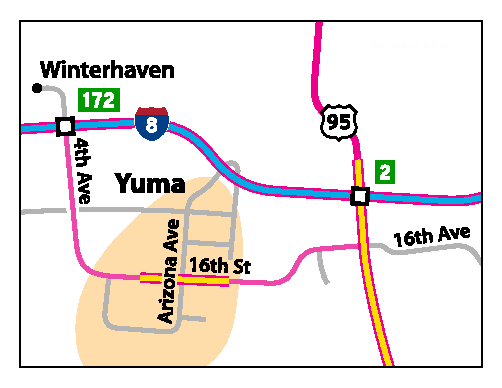
\includegraphics[scale=0.77]{cities/arizona/yuma}
\centering\caption{Street name map of Yuma, Arizona}
\end{figure}



\chapter{Idaho}
\City{Boise}

\begin{LocationList}

\Location{Charged}
On Technology~Way off \ID{21} Gowen~Rd, east in Boise.

\Location{Deepgrove \SpecialTransport}
On the south side of Federal~Way, off \ID{21} Gowen~Rd.
From \I{84} \Exit{57} turn north, then west.

\Location{Farmer's Barn}
On the east side of \ID{55} Eagle~Rd, by the railroad crossing.

\Location{\GarageHQ \Garage}
On Gowen~Rd. From \I{84} \Exit{57} follow signs for Gowen Field.

\Location{International \TruckDealer \Dealer \Rest \Service}
Between Gowen~Rd and Broadway~Ave, south in Boise.

\Location{Olthon Homes}
On Federal~Way off \ID{21} Gowen~Rd.
From \I{84} \Exit{57} turn north, then west.

\Location{Plaster \& Sons building construction}
Between \US{20} Front~St and \US{20} Myrtle~St in downtown Boise.

\Location{Plaster \& Sons house construction}
Accessed from Island Woods~Dr, off \ID{55} Eagle~Rd to the west.

\Location{\RecruitmentAgency \Recruitment}
Off Broadway~Ave opposite the truck stop.

\Location{\TruckStop \Gas \Rest \Service \Weigh}
On Broadway~Ave by \I{84} \Exit{54}.

\Location{Wallbert}
On Gowen~Rd. From \I{84} \Exit{57} follow signs for Gowen Field.

\end{LocationList}

\City{Coeur d'Alene}

\begin{LocationList}

\Location{Avalanche Steel}
Off \I{90} \Exit{11} to the north.

\Location{Deepgrove}
Accessed from \US{95} opposite Putnam~Rd, 40~miles south of Coeur d'Alene.

\Location{Drake Car Dealer}
By \US{95}, just north of \I{90} \Exit{12}.

\Location{\GarageHQ \Garage}
Off \I{90} \Exit{11} to the north.
Opposite the entrance to Avalanche Steel.

\Location{HMS Machinery}
On Seltice~Way, off Northwest~Blvd to the west.

\Location{Home Store}
Off \US{95}, northeast of \I{90} \Exit{12}.

\Location{Plaster \& Sons house construction}
In \Town{Fernan}[,] off \I{90} \Exit{15}.

\Location{Plaster \& Sons warehouse construction}
In the west of the commercial area north of \I{90} \Exit{11}.

\Location{\RecruitmentAgency \Recruitment}
Off \US{95}, northeast of \I{90} \Exit{12}.

\Location{Sea Horizon}
On Marina~Dr, off \US{95} south of Coeur d'Alene.

\Location{\TruckStop \Gas \Rest \Service}
On Coeur d'Alene Lake~Dr at Sherman~Ave, off \I{90} \Exit{15}.

\Location{Wallbert}
On Sherman~Ave at 15th~St, off \I{90} \Exit{15}.

\end{LocationList}

\City{Grangeville}

\begin{LocationList}

\Location{Coastline Mining}
Off \ID{13} to the south, just east of Grangeville.

\Location{Deepgrove sawmill}
On \US{95}, just north of Grangeville.

\Location{Deepgrove timber harvest site}
Off \US{12} to the north between \Town{Kooskia} and \Town{Kamiah}[.]

\Location{Farmer's Barn}
On County~Rd, accessed from \US{95} in the north of Grangeville.

\Location{HMS Machinery}
On County~Rd, accessed from \US{95} in the north of Grangeville.

\Location{Shop Town}
On \ID{13} Main~St.

\Location{Sunshine Crops}
Off \ID{13} to the south, just east of Grangeville.

\Location{\TruckStop \Gas \Rest}
At the intersection of \US{95} and \ID{13}.

\Location{Venture}
On \ID{13}, just east of Grangeville.

\end{LocationList}

\City{Idaho Falls}

\begin{LocationList}

\Location{Charged}
On Sunnyside~Rd, between Holmes~Ave and Yellowstone~Ave, just southeast of downtown.

\Location{Gallon Oil \UndergroundTank \Gas \Rest \Service \Weigh}
At the Phoenix truck stop by \I{15} \Exit{113}.

\Location{\GarageHQ \Garage \SpecialTransport}
Off \US{20}[Bus] Holmes Ave to the west.
Use \I{15} \Exit{119} and \US{20} \Exit{310}.

\Location{HMS Machinery}
By the airport, off \I{15} \Exit{119}.

\Location{Home Store}
On Holmes~Ave, between 7th~St and Sunnyside~Rd, in the southeast of Idaho Falls.

\Location{Peterbilt \TruckDealer \Dealer \Rest \Service}
By \I{15} \Exit{113}, opposite the Haulett truck stop.

\Location{Plaster \& Sons garage}
On Yellowstone~Ave, between Broadway~St and Sunnyside~Rd, just south of downtown.

\Location{Plaster \& Sons house construction}
On Rollandet~Ave, between 7th~St and Sunnyside~Rd, in the southeast of Idaho Falls.

\Location{\RecruitmentAgency \Recruitment}
On \US{20}, off \I{15} \Exit{118}.

%\Location{Special Transport \SpecialTransport}
%By the garage, off \US{20}[Bus] Holmes~Ave to the west. Use \I{15} \Exit{119} and \US{20} \Exit{310}.

\Location{Voltison Motors}
Off \US{20}[Bus] Holmes~Ave to the west, just north of the \US{26} junction.
Use \I{15} \Exit{119} and \US{20} \Exit{310}.

\end{LocationList}

\City{Ketchum}

\begin{LocationList}

\Location{Bitumen}
Accessed from Saddle~Rd, northwest in Ketchum.

\Location{Eddy's}
Southeast in Ketchum.

\Location{Plaster \& Sons}
In \Town{Sun Valley}[,] east of Ketchum.

\Location{Sell Goods}
Accessed from Saddle~Rd, northwest in Ketchum.

\end{LocationList}

\GasRestNote{The closest rest area is located at the junction of \ID{75} and \US{20}. A~truck stop offering gas is further south in \CityRef{Twin Falls}.}

\City{Lewiston}

\begin{LocationList}

\Location{AI Automotive}
By \US{12}, just northeast of downtown.

\Location{Avalanche Steel}
By the Page \& Price Paper plant. Accessed from \US{12} to the south, just east of downtown.

\Location{Farmer's Barn \SpecialTransport}
In the Port Districts, off \ID{128} at the Old Spiral Highway.

\Location{Page \& Price Paper}
Accessed from \US{12} to the south, just east of downtown.

\Location{Steeler}
In the Port Districts, off \ID{128} at the Old Spiral Highway.

\Location{Western Star \TruckDealer \Dealer \Gas \Rest \Service \Weigh}
At the truck stop on the joint section of \US{12} and \US{95}.

\end{LocationList}

\City{Nampa}

\begin{LocationList}

\Location{Darchelle Uzau}
On Chicken Dinner~Rd at \ID{55} Karcher~Rd, off \I{84}[Bus].
Use~\I{84} \Exit{38}.

\Location{Farmer's Barn}
On \ID{55} Karcher~Rd, off \I{84}[Bus].
Use \I{84} \Exit{38}.

\Location{Sunshine Crops}
On Can-ada~Rd at \US{20} \US{26} Chinden~Blvd, off \I{84} \Exit{38} to the north.

\Location{Wallbert}
Off Idaho Center~Blvd to the east, by \I{84} \Exit{38}.

\end{LocationList}

\GasRestNote{The closest truck stop with gas station and rest area is located in \CityRef{Boise} by \I{84} exit 54.}

\City{Pocatello}

\begin{LocationList}

\Location{Chemso}
Off \US{30} Garrett~Way, just south of \I{86} \Exit{58}.

\Location{Coastline Mining}
Accessed from Merrill~Rd, off \I{15} \Exit{47}.

\Location{Drake Car Dealer}
By McKinley~Ave, off \US{30} Gould~St to the southwest.

\Location{Plaster \& Sons}
By \I{15} \Exit{67}.
Turn north opposite the gas station, then take the next left turn.

\Location{Rail Export}
Off \US{30} Garrett~Way, south of \I{86} \Exit{58}.

\Location{Sunshine Crops \Rest}
Off \I{86} \Exit{58} to the north.

\Location{\TruckStop \Gas \Rest \Weigh}
Southwest of \I{86} \Exit{58}.

\end{LocationList}

\City{Salmon}

\begin{LocationList}

\Location{Bushnell Farms}
On \US{93}, just north of Salmon.

\Location{Coastline Mining}
Off \US{93} Main~St to the north, between the Salmon River bridge and the \ID{28} junction.

\Location{Drake Car Dealer}
On \US{93}, in the south of Salmon.

\Location{Farmer's Barn}
On \ID{28}.

\Location{\GarageHQ \Garage}
Off \US{93}, in the north of Salmon.

\Location{\GasStation \Gas \Rest}
The NAF on \US{93}.

\Location{Wallbert}
North of the junction of \US{93} and \ID{28}.

\end{LocationList}

\City{Sandpoint}

\begin{LocationList}

\Location{Coastline Mining \Rest \Weigh}
On Baldy Mountain Road.
From \US{2} \US{95} take Schweitzer Cutoff west, then turn south at the roundabout.

\Location{Deepgrove \Multiple \Rest}
Off Baldy Mountain Road (sawmill with rest area to the south, logging site to the north).
From \US{2} \US{95} take Schweitzer Cutoff west, then turn south at the roundabout.

\Location{Farmer's Barn}
At the end of Schweitzer Cutoff, west of \US{2} \US{95}.

\Location{HMS Machinery \Rest}
On Baldy Mountain Road.
From \US{2} \US{95} take Schweitzer Cutoff west, then turn south at the roundabout.

\Location{Home Store}
On Kootenai Cutoff, east of \US{2} \US{95}.

\Location{Plaster \& Sons}
North of Schweitzer Cutoff, off \US{2} \US{95} to the west.

\Location{\TruckStop \Gas \Rest}
At \US{2} \US{95} and Schweitzer Cutoff.

\Location{Wallbert}
On Larch Street, off \US{2} to the west.

\end{LocationList}

\City{Twin Falls}

\begin{LocationList}

\Location{Coastline Mining cement plant}
On \US{30} \US{93}[Bus] Addison~Ave.

\Location{Coastline Mining storage \Weigh}
Off \US{93}, just north of the \US{30} interchange.

\Location{\GarageHQ \Garage}
On Eastland~Dr at Kimberly~Rd, in the southeast of Twin Falls.

\Location{Haulett \UndergroundTank \Gas \Rest \Service \Weigh}
At the Haulett truck stop, off \US{93} by \I{84} \Exit{173}.

\Location{Home Store}
On the east side of \US{93}[Bus] Blue Lakes~Blvd.

\Location{Mack \TruckDealer \Dealer \Rest \Service}
On Kimberly~Rd at Eastland~Dr, in the southeast of Twin Falls.

\Location{Plaster \& Sons}
On Elizabeth~Blvd at Eastland~Dr, in the east of Twin Falls.

\Location{\RecruitmentAgency \Recruitment}
On Eastland~Dr, in the east of Twin Falls.

\Location{Sunshine Crops \SpecialTransport}
On 3700~N, off \US{93} southwest of Twin Falls.

\Location{Venture}
On Orchard~Dr, southwest of downtown.

\Location{Wallbert}
On Fillmore~St, off \US{93}.

\end{LocationList}



\chapter{Washington}
\City[aberdeen_wa]{Aberdeen}

\begin{LocationList}

\Location{Bitumen}
On Myrtle~St between Aberdeen and \Town{Hoquiam}[,] west of \US{101}.

\Location{Deepgrove depot}
Southwest of downtown Aberdeen by the port.
Take Park~St, then turn right at the end.

\Location{Deepgrove timber harvest site}
Accessed from \US{101} about 4~miles south of the city center.

\Location{Eddy's}
On Wishkah~St at H~St.

\Location{Page \& Price Paper}
Off \US{101} to the east, at the southern city limit of Aberdeen.

\Location{Sea Horizon \Rest}
Southwest of downtown Aberdeen by the port.
Take Park~St, then turn right at the end.

\end{LocationList}

\GasRestNote{The closest truck stop with a gas station is located by \I{5} south of \CityRef{Olympia}.}

\City{Bellingham}

\begin{LocationList}

\Location{Deepgrove logging site}
On Mount Baker,
% (which appears by name on a sign in Wickersham)
between \Town{Wickersham} and \Town{Newhalem}[.]
Accessed from \WA{20}, 30~miles east of \I{5}.

\Location{Deepgrove sawmill}
By the airport, off \I{5} \Exit{258}.

\Location{Fish Tail Foods}
In Bellingham Port.
Follow signs for the airport from \I{5} \Exit{258}, then turn south after the sawmill.

\Location{International \TruckDealer \Dealer \Rest \Service}
Off Iowa~St to the north, east of \I{5} \Exit{254}.

\Location{\RecruitmentAgency \Recruitment}
Off Iowa~St to the north, east of \I{5} \Exit{254}.

\Location{Sea Horizon}
In Bellingham Port.
From the city center, head west on Holly~St, then turn south.

\Location{Sell Goods}
Off Iowa~St to the north, east of \I{5} \Exit{254}.

\Location{\TruckStop \Gas \Rest}
By \I{5} \Exit{258}.

\Location{Wallbert}
At Bakerview~Rd and Arctic~Ave, north of \I{5} \Exit{258}.

\end{LocationList}

\City{Colville}

\begin{LocationList}

\Location{Bushnell Farms}
Accessed from \US{395}, 30~miles south of Colville.

\Location{Coastline Mining}
Off \WA{20} 3rd~Ave.

\Location{Deepgrove}
Off Railroad~St, by the northwestern roundabout.

\Location{Eddy's}
East of \US{395} Main~St, by the southern roundabout.

\Location{Gallon Oil \UndergroundTank \Gas \Rest}
At the Gallon Oil truck stop on \US{395} \WA{20} Main~St.

\Location{Sea Horizon}
Accessed from \US{395}, 30~miles south of Colville.

\Location{Sell Goods}
On Railroad~St, west of \US{395} Main~St by the southern roundabout.

\Location{Sunshine Crops}
On 3rd~Ave, off Railroad~St to the west.
There are two Sunshine Crops facilities here.
A garage is to the right, a farm to the left.

\end{LocationList}

\City{Everett}

\begin{LocationList}

\Location{Avalanche Steel}
By the southbound lanes of \WA{529} Broadway.

\Location{Darwing}
Off \WA{526} Darwing~Fwy.

\Location{\GasStation \Gas}
On \WA{529} at Everett~Ave and Broadway, in the city center.

\Location{HMS Machinery}
Next to Avalanche Steel, by the southbound lanes of \WA{529} Broadway.

\Location{\RestArea \Rest}
On \WA{529} Broadway, next to the gas station.

\Location{Sea Horizon}
By the Port of Everett.
From the city center, head west on Everett~Ave.

\Location{Sell Goods}
In the Port of Everett.
From the city center, head west on Everett~Ave.

\Location{Shop Town}
On \WA{529} Everett~Ave at Broadway, in the city center.

\end{LocationList}

\City{Grand Coulee}

\begin{LocationList}

\Location{Coastline Mining}
East of \WA{155}, one block north of the Tidbit by the river bridge.

\Location{Gallon Oil \UndergroundTank \Gas}
At the Aron gas station on \WA{155}, by the \WA{174} junction.

\Location{Plaster \& Sons}
One block east of the bridge carrying \WA{155} across the river.

\Location{\RestArea \Rest}
On \WA{155}, uphill from the generating plant at the dam.

\Location{Tidbit}
On \WA{155}, at the east end of the river bridge.

\end{LocationList}

\City{Kennewick}

\begin{LocationList}

\Location{Coastline Mining}
On Argent~Rd, off \I{182} \Exit{12} to the northwest.

\Location{\GarageHQ \Garage}
On 27th~Ave at \WA{397} Gum~St.

\Location{Home Store}
On Quillan~St at 27th~Ave.

\Location{Plaster \& Sons}
On 27th~Ave at the railroad crossing.

\Location{Rail Export}
Off \WA{397} to the east, just north of the Ed~Hendler Bridge.

\Location{Sunshine Crops}
On Kartchner~St, off \US{395} north of Kennewick.

\Location{\TruckStop \Gas \Rest \Weigh}
By the Kartchner~St exit off \US{395}, north of Kennewick.

\Location{Wallbert market}
On Quillan~St, south of 27th~Ave.

\Location{Wallbert warehouse}
On \WA{397} Gum~St at 27th~Ave.

\end{LocationList}

\City[longview]{Longview}

\begin{LocationList}

\Location{Deepgrove sawmill}
On the West Docks in Port Longview, off \WA{433}.

\Location{Deepgrove timber harvest site}
Accessed from \US{12}, 25~miles from \I{5} \Exit{68}.

\Location{\GasStation \Gas}
At the intersection of \WA{432} and \WA{433}.

\Location{Page \& Price Paper}
On the East Docks in Port Longview, off \WA{433}.

\Location{\RestArea \Rest}
On the south side of \WA{432}, by \I{5} \Exit{36}.

\end{LocationList}

\City{Olympia}

\begin{LocationList}

\Location{Coastline Mining}
On Britton~Pkwy, off \I{5} \Exit{111} to the northwest.

\Location{Deepgrove}
On Franklin~St at Olympia~Ave, in the Port of Olympia northwest of the city center.

\Location{Enterpriser}
On Marvin~Rd, off \I{5} \Exit{111} to the northwest.

\Location{\GarageHQ \Garage}
On Willamette~Dr, off \I{5} \Exit{111} to the northwest.

\Location{Home Store}
In West Olympia, by the \US{101} interchange.

\Location{\RecruitmentAgency \Recruitment}
On Marvin~Rd, off \I{5} \Exit{111} to the northwest.

\Location{Sea Horizon}
On Franklin~St at Olympia~Ave, in the Port of Olympia northwest of the city center.

\Location{Sell Goods}
On Willamette~Dr, off \I{5} \Exit{111} to the northwest.

\Location{Shop Town}
In West Olympia, by the \US{101} interchange.

\Location{Steeler}
On Marvin~Rd, off \I{5} \Exit{111} to the northwest.

\Location{\TruckService \Service}
On Marvin~Rd, off \I{5} \Exit{111} to the northwest.

\end{LocationList}

\GasRestNote{Truck stops with gas stations and rest areas are located close by on \I{5} in either direction.}

\City{Omak}

\begin{LocationList}

\Location{Eddy's}
Off \US{97}[Bus] Riverside~Dr, opposite the truck stop.

\Location{Gallon Oil \UndergroundTank \Gas \Rest}
At the Gallon Oil truck stop on \US{97}[Bus] Riverside~Dr.

\Location{Sunshine Crops \SpecialTransport}
Accessed from \WA{20}, just west of Omak.

\end{LocationList}

\City{Port Angeles}

\begin{LocationList}

\Location{Apade}
In northeastern Port Angeles, north of \US{101}.
From \US{101} Lincoln~St, turn onto \US{101} First~St, then take the next left turn.

\Location{Avalanche Steel}
In the industrial area off \US{101}, just southwest of Port Angeles.
Go straight.

\Location{Coastline Mining}
In the industrial area off \US{101}, just southwest of Port Angeles.
Turn right.

\Location{Deepgrove}
In the industrial area off \US{101}, just southwest of Port Angeles.
Take the second right turn.

\Location{\GasStation \Gas \Rest}
On Marine~Dr by the harbour, west of the truck route.

\Location{HMS Machinery}
At the southwestern end of Tumwater Truck~Rd, in the one-way section.

\Location{Lumen Auto}
On \US{101} East First~St.

\Location{Page \& Price Paper}
At the far end of Marine~Dr, northwest of Port Angeles.

\Location{Sea Horizon \SpecialTransport}
On Tumwater Truck~Rd at Marine~Dr, just west of downtown.

\Location{Tidbit}
On \US{101} at the intersection of First~St and Lincoln~St.

\Location{\TruckService \Service \Rest}
On the waterfront at Lincoln~St, opposite the \q{Landing.}

\end{LocationList}

\City{Seattle}

\begin{LocationList}

\Location{Avalanche Steel}
On 4th~Ave, off \I{5} \Exit{163}.

\Location{Coastline Mining}
South of Spokane~St near the port, off \I{5} \Exit{163}.

\Location{\GarageHQ \Garage}
On Southport~Dr, by \I{405} \Exit{5}.

\Location{Kenworth factory \Rest}
At Garden~Ave and 6th~St.
Take \I{405} \Exit{5} for Southport~Dr / Park~Ave.
Turn left onto Garden~Ave, then left again.

\Location{Kenworth \TruckDealer \Dealer \Rest \Service}
On 4th~Ave, off \I{5} \Exit{163}.

\Location{Port of Seattle \SpecialTransport}
Off \I{5} \Exit{163}.

\Location{Rail Export}
On 4th~Ave, off \I{5} \Exit{163}.

\Location{\RecruitmentAgency \Recruitment}
On 1st~Ave, off \I{5} \Exit{163}.

\Location{Wallbert}
On \WA{900} Sunset~Blvd, off \I{405} \Exit{5}.
Use the left lane.

\end{LocationList}

\GasRestNote{The closest truck stop with a gas station is located in \CityRef{Tacoma}, on \I{5} to the south.}

\City{Spokane}

\begin{LocationList}

\Location{Coastline Mining}
By \US{2} roughly 60~miles west of Spokane. % (25~miles east of \Town{Coulee City})

\Location{\GarageHQ \Garage}
On Trent~Ave, northwest of the truck stop.

\Location{Haulett \UndergroundTank \Gas \Rest \Service \Weigh}
At the Haulett truck stop by \I{90} \Exit{286}.

\Location{Home Store}
On Frederick~Ave at Broadway~Ave, off \I{90} \Exit{286} to the north.

\Location{Plaster \& Sons}
Off Spokane Falls~Blvd to the north, just east of downtown.
Use~\I{90} \Exit{281}.

\Location{Rail Export \SpecialTransport}
Accessed from Frederick~Ave.
Take \I{90} \Exit{286} and head north.
Turn right onto Frederick, then right again.

\Location{Steeler}
On Frederick~Ave at Broadway~Ave, off \I{90} \Exit{286} to the north.
Use the left lane.

\Location{Voltison Motors}
Between Browne~St and Division~St in downtown Spokane.
Take~\I{90} \Exit{281}, then take the first left turn.

\Location{Volvo \TruckDealer \Dealer \Rest \Service}
On North River~Dr at \US{2} \US{395} Division~St.

\Location{Wallbert}
On the east side of Division~St, just south of the \US{2} / \US{395} split.

\end{LocationList}

\City{Tacoma}

\begin{LocationList}

\Location{Drake Car Dealer}
On 20th Street, off \I{5} \Exit{136}[A].

\Location{Gallon Oil}
Opposite the entrance to the Port of Tacoma, off \I{5} \Exit{136}[B].

\Location{HMS Machinery}
On 20th Street, off \I{5} \Exit{136}[A].

\Location{Peterbilt \TruckDealer \Dealer \Rest \Service}
On 20th Street, off \I{5} \Exit{136}[A].

\Location{Phoenix \UndergroundTank \Gas \Rest \Weigh}
At the Phoenix truck stop on Port of Tacoma~Rd, by \I{5} \Exit{136}[B].

\Location{Port of Tacoma}
Off \I{5} \Exit{136}[B].

\Location{Wallbert}
On 20th Street, off \I{5} \Exit{136}[A].

\end{LocationList}

\City{Vancouver}

\begin{LocationList}

\Location{Charged}
On Grand~Blvd, off \WA{14} \Exit{1} to the north.

\Location{Coastline Mining}
On Brady~Rd at 192nd~Ave, off \WA{14} \Exit{10}.

\Location{\GasStation \Gas}
On Columbia House~Blvd at Grove~St, off \WA{14} \Exit{1}.

\Location{Steeler \Multiple}
On Columbia~Way, off \WA{14} \Exit{1}.
There are two Steeler facilities here: a workshop and a warehouse around the back.

\Location{Tidbit}
On Columbia House~Blvd at Grand~Blvd, off \WA{14} \Exit{1} to the north.

\end{LocationList}

\GasRestNote{Rest areas can be found across the river in \Town{Portland}[.]}



\TODO{fix CityRef Portland}

\City{Wenatchee}

\begin{LocationList}

\Location{Bushnell Farms}
In \Town{Orondo} by \US{2} \US{97}, northeast of Wenatchee.

\Location{Enterpriser}
By \US{2} \US{97} northeast of Wenatchee.
Follow signs for the Gallon Oil truck stop.

\Location{Gallon Oil \UndergroundTank \Gas \Rest \Service}
At the Gallon Oil truck stop signed from \US{2} \US{97} northeast of Wenatchee.

\Location{\GarageHQ \Garage}
At the signalled intersection on \US{2} \US{97} just east of the \WA{285} interchange.

\Location{HMS Machinery}
In downtown Wenatchee, east of the railroad tracks.
From \WA{285} turn onto Hawley~St, then take the next right turn.

\Location{\RecruitmentAgency \Recruitment}
On Miller~St, in downtown Wenatchee.

\Location{Sell Goods}
In downtown Wenatchee, east of the railroad tracks.
From \WA{285} turn onto Hawley~St, then take the next right turn.

\Location{Starbridge}
Accessed from \US{2} \US{97} northeast of Wenatchee.
Follow signs for the Gallon Oil truck stop.

\Location{Tidbit}
On Orondo~Ave at Wenatchee~Ave, in downtown Wenatchee.
Use~the left lane.

\Location{Venture}
Accessed from \US{2} \US{97} northeast of Wenatchee.
Follow signs for the Gallon Oil truck stop.

\end{LocationList}

\City{Yakima}

\begin{LocationList}

\Location{Bitumen}
In \Town{Union Gap}[,] off Main~St to the west.
Use \I{82} \Exits{37}{38}.

\Location{Bushnell Farms}
Between \Town{Union Gap} and \Town{Goldendale}[,] by \US{97} 25~miles south of Yakima.

\Location{Coastline Mining \Weigh}
In \Town{Ellensburg}[,] accessed from \US{97} 45~miles north of Yakima.

\Location{Gallon Oil \UndergroundTank \Gas \Rest \Service \Weigh}
At the Gallon Oil truck stop on Rudkin~Rd, between Valley Mall~Blvd and Yakima~Ave.

\Location{Global Mills}
Off 1st~St to the west.
Use \I{82} \Exit{31}[B].

\Location{Mack \TruckDealer \Dealer \Rest \Service}
By the Global Mills plant, off 1st~St to the west.

\Location{Rail Export}
In \Town{Union Gap}[,] off Main~St to the west.
Use \I{82} \Exits{37}{38}.

\Location{\RecruitmentAgency \Recruitment}
By the Global Mills plant, off 1st~St to the west.

\Location{Sunshine Crops}
Off \US{12} to the south in \Town{Naches}[,] 10~miles west of Yakima.

\Location{Wallbert}
In \Town{Union Gap}[,] on Valley Mall~Blvd at Main~St.
Use \I{82} \Exits{37}{38}.

\end{LocationList}



\end{document}
